\documentclass[spanish,twocolumn]{article}
\usepackage{spconf,amsmath,graphicx}
\usepackage{mathptmx}
\usepackage{mathtools}
\usepackage{amsmath}
\usepackage{mathrsfs}
\usepackage{amssymb}
\usepackage{amsfonts}
\usepackage[utf8]{inputenc}
\usepackage{babel}
\usepackage{color}
\usepackage[Algoritmo]{algorithm}
\usepackage{algpseudocode}
\usepackage{multicol}
\usepackage{caption,setspace}
\usepackage{subfig}
\usepackage{graphicx}

\algrenewcommand\algorithmicif{\textbf{si}}
\algrenewcommand\algorithmicend{\textbf{fin}}
\algrenewcommand\algorithmicfor{\textbf{para}}
\algrenewcommand\algorithmicdo{\textbf{hacer}}
\algrenewcommand\algorithmicwhile{\textbf{mientras}}
\algrenewcommand{\algorithmicrequire}{\textbf{Entrada:}}
\algrenewcommand{\algorithmicensure}{\textbf{Salida:}}
\selectlanguage{spanish}

\def\x{{\mathbf x}}
\def\L{{\cal L}}

\title{OPTIMIZACIÓN MULTIOBJETIVO (FALTA CREAR TITULO) }

\name{Monserrat Mora, Adriana Coronel, Diego Pinto-Roa, José Luis Vázquez Noguera}
\address{Facultad Politécnica - Universidad Nacional de Asunción}

\begin{document}
%	
\maketitle
%
\begin{abstract}

% acá va a ir en unas 2 líneas el problema que se plantea
% la mejora del contraste está relacionada con las métricas que se utilizan para medir la cantidad de información y la calidad de la imagen.
% es necesario que las métricas sean contradictorias para resolver el problema 
% se propone un enfoque de comparación basado en la correlación de pearson para medir la relación inversa entre métricas.
% Los resultados muestran que una dupla de métricas obtiene el coeficiente más bajo de correlación, lo que indica que son los objetivos más contradictorios.

La mejora de contraste en imágenes en escala de gris es una técnica que busca resaltar la información útil de la imagen. Las técnicas, por lo general están relacionadas con las métricas que se utilizan para medir la cantidad de información y la calidad de la imagen. Escoger las métricas adecuadas de forma a lograr maximizar la información disponible minimizando la cantidad de ruido introducido supone un paso fundamental para lograr resultados en el proceso. En este trabajo se propone un enfoque de comparación basado en la Correlación de Pearson para medir la proporción de cambio inversa entre métricas.Los resultados muestran que una dupla de métricas obtiene el coeficiente más bajo de correlación, lo que indica que los objetivos muestran mayor correlación inversa y por lo tanto son las mejores métricas para utilizar dentro del algoritmo de mejora de contraste. Se realizaron comparaciones de a pares entre Entropía, Entropía Local, Índice de Similitud Estructural y la métrica Local Tuned Global.

%Los objetivos propuestos son maximizar la cantidad de información disponible (Entropía / Entropía local) y minimizar la distorsión en las imágenes resultantes (por medio del Índice de Similitud Estructural y el modelo Local Tuned Global) de manera simultánea.

\end{abstract}
%
\begin{keywords}
SMPSO, CLAHE, Entropía, Entropía Local, SSIM, LTG, Mejora del Contraste, Optimización.
\end{keywords}
%
\section{Introducción}
\label{sec:intro}

Las imágenes digitales están expuestas a sufrir una variedad de distorsiones durante su procesamiento, compresión, almacenamiento, transmisión y reproducción, y cualquiera de ellas puede resultar en la degradación de la calidad visual.

El principal objetivo de las técnicas de mejora es procesar una imagen de forma que resulte más adecuada que la original para una aplicación específica. Existen muchas técnicas de Mejoras de Contraste en el procesamiento de imágenes usadas para mejorar la apariencia de una imagen y hacerla más apta para la percepción visual humana. Una estrategia fundamental para la mayoría de las técnicas de Mejora de Contraste es la transformación del histograma. La técnica más usadas debido a su simplicidad y eficienca es la Ecualización del Histograma (HE). 	

Es de gran importancia realizar la Mejora del Contraste de imágenes de carácter médico, debido a que de esta manera es posible acentuar y mantener las características presentes en ellas. Las radiografías presentan características particulares de contraste, como en el caso de radiografías del tórax y mamografías, donde pueden existir diferencias de constraste notorias debido a las características de atenuación de los Rayos X \cite{chang1998image}.

Los enfoques de mejora local demuestran ser sumamente útiles al momento de realzar detalles en imágenes médicas, y existen diversas propuestas que se centran en mejorar el contraste en radiografías \cite{1625082,4712472,5360176}. Debido a ello en esta  propuesta se estudia la comparación de la correlación de entre dos metricas, la entropía local vs. SSIM y la entropía local vs LTG.

 utilizará una metaheurística de optimización de objetivos, de manera a sintonizar los parámetros de entrada del algoritmo de mejora del contraste descripto en la sección \ref{sec:clahe}, de manera a obtener un grupo de imágenes contrastadas, las cuales serán evaluadas en cuanto a la ganancia de información proveída y distorsión introducida por la ecualización (sección \ref{sec:metricas}).

\section{Contrast Limited Adaptive Histogram Equalization (CLAHE)}
\label{sec:clahe}
Este enfoque de mejora de contraste presentado en \cite{Zuiderveld:1994:CLA:180895.180940} es una extensión del algoritmo original Adaptive Histogram Equalization (AHE) \cite{pizer1987adaptive}; en ambos métodos se implementa una Ecualización del Histogama basada en {\it Regiones Contextuales} cuyas dimensiones están delimitadas por $(\mathcal{R}_x, \mathcal{R}_y)$, para realizar la ecualización en varios sectores de la imagen. Las inconsistencias entre fronteras de la imagen se corrigen aplicando interpolación bilineal. AHE presenta problemas de amplificación del ruido, entonces en CLAHE se implementa una limitación en el contraste a través de la limitación de la cantidad de pixeles que pueden alcanzar cierto nivel de gris dentro del histograma local; aquí se define el coeficiente {\it Clip Limit} $\mathcal{C}$ como un factor que está fuertemente relacionado con los contenidos del histograma. 

\section{métricas de evaluación}
\label{sec:metricas}

Se adoptan tres métricas consideradas importantes para las comparaciones de los resultados optenidos por el CLAHE que nos permitan determinar cuantitativamente la calidad de las mismas; éstas son la Entropia local como medida de mejora del contraste, el Índice de Similitud Estructural y el modelo Local Tuned Globa como medidas de distorsión de la imagen.

\subsection{Entropía}
\label{ssec:entropia}

La {\it Entropía de la Información} es una medida de la aleatoriedad presente en la imagen \cite{tsai2008information}. Se puede definir la Entropía de la imagen como: 

\begin{equation}\label{eq:entropia}
\mathscr{H}=-\sum_{i=0}^{L-1}\mathcal{P}_i log_2(\mathcal{P}_i) [bits] \quad \mathscr{H} \in {0,..,log_2(L)} 
\end{equation}

Donde $\mathcal{P}_i$ es la probabilidad de ocurrencias del nivel de gris $i$ en el histograma y $L$ es el máximo nivel de gris que se puede utilizar para representar la imagen. Esta métrica es interesante debido a que está fuertemente asociada al brillo medio de la imagen \cite{108593}; este coeficiente nos ayuda a ver cuánto aumenta el contraste como consecuencia de la transformación de la imagen.


\subsection{Índice de similitud estructural (SSIM)}
\label{ssec:ssim}
El {Índice de Similitud Estructural (SSIM)} \cite{wang2004image} es un coeficiente que mide el grado de distorsión producida en una imagen resultante $T$ a consecuencia de aplicar una Mejora del Contraste a una imagen original $I$. SSIM se calcula por bloques, por lo que si definimos dos ventanas $I_x$ e $T_y$ para las imágenes original y resultante, respectivamente, se define el SSIM como se muestra abajo:

\begin{equation}\label{eq:ssim}
\resizebox{.9\hsize}{!}
{
$SSIM(I,T)=\frac{(2\mu_{I_x}\mu_{T_y}+C_1)(2\sigma_{I_xT_y}+C_2)}{(\mu_{I_x}^2+\mu_{T_y}^2+C_1)(\sigma_{I_x}^2+\sigma_{T_y}^2+C_2)} \quad SSIM \in [0,1]$
}
\end{equation}

Donde $\mu_{I_x}$ es el promedio de intensidades de $I_x$; $\mu_{T_y}$ es el promedio de intensidades de $T_y$; $\sigma_{I_x}^2$ y $\sigma_{T_y}^2$ son las varianzas de intensidades de $I_x$ e $T_y$, respectivamente; $\sigma_{I_x T_y}$ es la covarianza entre $I_x$ e $T_y$; $C_1=(K_1L^2)$, $L$ es el rango dinámico de intensidades de los pixeles (256 para una imagen en escala de grises de 8 bits) y $K_1 \ll 1$ es una constante pequeña; $C_2=(K_2 L)^2$, y $K_2 \ll 1$; tanto $C_1$ y $C_2$ son constantes que se usan para estabilizar la division en caso de que el denominador tienda a cero.

\subsection{ Local Tuned Global Model (LTG)}
\label{ssec:ltg}
El modelo {Local Tuned Global (LTG)} está inspirado en las metricas IQA (Image Quality Assessment), fue introducido bajo la hipotesis de que la percepción visual humana en  la calidad de la imagen depende de la distorsión local resaltante y la degradación global de la calidad. %falta citación del ltg, mencionar que es un enfoque basado en gradiente de la imagen y citar
El modelo extrae información sobre la luminancia (brillo percibido por el ojo humano) y la crominancia (información del color) de la imagen de entrada y la imagen distorsionada, luego mide la distorsión local resaltante y la degradación global de la calidad en la información obtenida sobre la luminancia y compara las diferencias en la informacion obtenida sobre la crominancia, derivando así el valor global de la calidad de la imagen.

\begin{equation}\label{eq:ltg}
\resizebox{.6\hsize}{!}
{
$LTG(x,y) =\frac{\Phi(G_{s}^{\theta_1})}{\Phi(G_{m}^{\theta_2})} \Phi(I_{m}^{\theta_3}.Q_{m}^{\theta_3})$
}
\end{equation}

Donde:
\begin{itemize}
 \item $G_{m}$ = es el gradiente %citar gradiente 
  medio de la imagen original y distorsionada.
 \item $ G_{s}$ = indica los pixeles con valores S\% más altos en $G_{m}$.
 \item  $I_{m}$ y $Q_{m}$ = contienen la información de crominancia de las imagenes. 
\end{itemize} 

%vamos a mencionar un poquito lo que es el coeficiente de correlación de pearson

\section{Formulación del Problema Planteado}
\label{sec:formulacion}

Dadas la imagen de entrada $I$, y un vector $\overrightarrow{x}=(\mathcal{R}_x, \mathcal{R}_y, \mathcal{C})$, donde $\mathcal{R}_x$ y $\mathcal{R}_y$ conforman la región contextual y $\mathscr{C}$ es el $Clip Limit$, se desea calcular el conjunto de soluciones $\mathscr{X}$ que maximice de manera simultánea los objetivos $f_1$ y $f_2$, como se muestra abajo:

\begin{equation}\label{eq:fitness}
    f(I, \overrightarrow{x}) = \{ f_1(I, \overrightarrow{x}), f_2(I, \overrightarrow{x}) \} \qquad f_1,f_2 \in [0,1]
\end{equation}

donde:
\begin{itemize}
%\item $\overrightarrow{x}=(\mathcal{R}_x, \mathcal{R}_y, \mathcal{C})$, donde $\mathcal{R}_x$ y $\mathcal{R}_y$ conforman la región contextual y $\mathscr{C}$ es el Clip Limit.
\item $f_{1}(I, \overrightarrow{x})=\frac{\mathscr{H}(T)}{log_{2}L}$ es la Entropía local normalizada de la imagen $T$.
\item $f_{2}(I, \overrightarrow{x})=SSIM(I,T)$ es el Índice de Similitud Estructural o  el modelo Local Tuned Global  entre $I$ y $T$.

Siendo $T$ la imagen mejorada por $CLAHE(\overrightarrow{x},I)$ con los parámetros dados por $\overrightarrow{x}$ aplicados a $I$.

\end{itemize}

sujeto a:

\begin{itemize}
\item $\mathcal{R}_x \in [2,..,M]$ en los números $\mathbb{N}$.
\item $\mathcal{R}_y \in [2,..,N]$ en los números $\mathbb{N}$.
\item $\mathscr{C} \in (0,1]$ en los números $\mathbb{R}$.
\end{itemize}

Ésto significa que los valores de $\mathcal{R}$ solamente pueden tomar valores enteros positivos entre $(2,2)$ y $(M,N)$ y que $\mathscr{C}$ puede tomar un valor mayor a cero y menor o igual a 1.


\begin{algorithm}[H]
    \scriptsize
    \begin{algorithmic}[1]
        \Require imagen de entrada $I$, número de partículas $\Omega$, número de iteraciones $t_{max}$
        \State Inicializar los parámetros $\omega$, $C_1$, $C_2$, $t=0$, $lower\_limit_1$, $lower\_limit_2$, $lower\_limit_3$, $upper\_limit_1$, $upper\_limit_2$, $upper\_limit_3$, $\mathscr{X}$
        %\For{cada $i$-ésima partícula del enjambre}
        %    \State Inicializar la posición $x_i$ aleatoriamente
        %    \State Inicializar la velocidad $v_i$ a 0
        %    \State ${imagenMejorada}$ = CLAHE(${x_i}$, ${imagenOriginal}$)
        %    \State ${f_i}$ = evaluarAptitud(${imagenOriginal}$, ${imagenMejorada}$)
        %    \State Establecer el mejor individual inicial $p_i$ por el valor inicial $x_i$
        %    \If{$f_i < f_{p_g}$}
        %        \State reemplazar $p_g$ por el valor de $x_i$
        %    \EndIf
        %\EndFor
        \While{$t$ $<$ $t_{max}$}
            \For{cada $i$-ésima partícula del enjambre}
                \State Calcular la nueva velocidad de la partícula $\overrightarrow{v_i}^t$ utilizando la ecuación \eqref{eq:psobasico2}, sujeto a las restricciones impuestas por \eqref{eq:restricciondelta}

%                \begin{equation*}\label{eq:psobasico2}
%                    \overrightarrow{v_i}(t) = \omega \cdot \overrightarrow{v_i} \cdot (t-1) + C_1 \cdot r_1 \cdot (\overrightarrow{x_{p_i}}-\overrightarrow{x_i}) + C_2 \cdot r_2
%                \end{equation*}



                \State Calcular la nueva posición de la partícula $\overrightarrow{x_i}^t$ con la expresión de posición \eqref{eq:psobasico}
                %\begin{equation*}\label{eq:psobasico}
                %    \overrightarrow{x_i}(t) = \overrightarrow{x_i}(t-1) + \overrightarrow{v_i}(t)
                %\end{equation*}

                \State ${T}$ = CLAHE(${\overrightarrow{x_i}^t}$, ${I}$)
                \State ${f^t_i}$ = $f(I, \overrightarrow{x_i}^t)$%evaluarAptitud(${I}$, ${T}$)
                \If{$f^t_i < f_{\overrightarrow{x}_{p_i}}$}
                    \State reemplazar $\overrightarrow{x}_{p_i}$ por el nuevo valor de $\overrightarrow{x_i}^t$
                \EndIf
                \If{$ \overrightarrow{x_i} \succ \overrightarrow{x_{g_i}}$  }
                    \State actualizar $\mathscr{X}$
                \EndIf
                \State $t$ = $t$ + 1
            \EndFor
        \EndWhile
    \Ensure $\mathscr{X}$
    \end{algorithmic}
    \caption{Algoritmo $PSO-CLAHE$ Multiobjetivo.}
    \label{alg:pso_clahe}
\end{algorithm}

\section{propuesta}
\label{sec:propuesta}
Se utiliza el algoritmo $SMPSO$ \cite{4938830}, donde las soluciones potenciales $\overrightarrow{x}=(\mathcal{R}_x, \mathcal{R}_y, \mathcal{C})$ se denominan {\it partículas} y el conjunto de partículas $\Omega$ se denomina {\it enjambre}. Cada partícula $\overrightarrow{x_i}$ se actualiza en cada generación $t$ de acuerdo a la siguiente ecuación:

\begin{equation}\label{eq:psobasico}
\overrightarrow{x_i}^t = \overrightarrow{x_i}^{(t-1)} + \overrightarrow{v_i}^t
\end{equation}

donde el factor $\overrightarrow{v_i}$ se conoce como la velocidad y está dado por:

\begin{equation}\label{eq:psobasico2}
\overrightarrow{v_i}^t = \omega \cdot \overrightarrow{v_i}^{(t-1)} + C_1 \cdot r_1 \cdot (\overrightarrow{x_{p_i}}-\overrightarrow{x_i}) + C_2 \cdot r_2 \cdot (\overrightarrow{x_{g_i}}-\overrightarrow{x_i})
\end{equation}

Aquí, $\overrightarrow{x_{p_i}}$ es la mejor solución que encontró $\overrightarrow{x_i}$, $\overrightarrow{x_{g_i}}$ es la mejor partícula (también conocida como {{\it líder}) que se encuentra en todo el enjambre, $\omega$ es el peso de la inercia de la partícula, $r_1$ y $r_2$ son dos números aleatorios, y $C_1$ y $C_2$ son parámetros que controlan el efecto de las partículas locales  y globales. Si una partícula es mejor que otra, se dice que la $domina$, y la dominancia está definida de la siguiente manera: $\overrightarrow{x_{g_i}} \succ \overrightarrow{x_i}$ si y sólo si

\begin{equation}\label{eq:dominanciapareto}
         \begin{cases}  f_i(I,\overrightarrow{x_{g}})  \geq f_i(I,\overrightarrow{x}) \forall i \in \{1,2\} \\
                        f_i(I,\overrightarrow{x_{g}}) > f_i(I,\overrightarrow{x}) \exists i \in \{1,2\} \\
         \end{cases}
\end{equation}

El {\it Conjunto Pareto} es el grupo de soluciones $\mathscr{X}$, y la imagen en el espacio objetivo es el {\it Frente Pareto}.

En adición, en $SMPSO$ se realiza una restricción en $\overrightarrow{v}$, para cada componente $j$ de $\overrightarrow{x}$, de acuerdo a la siguiente ecuación: 
                
\begin{equation}\label{eq:restricciondelta}
    v_{i,j}^t = \begin{cases}  delta_j &\mbox{if } v_{i,j}^t > delta_j \\
                                -delta_j & \mbox{if } -delta_j \\
                                v_{i,j}^t & otherwise \end{cases}
\end{equation}

donde: 
\begin{equation} \label{eq:restricciondelta2}
delta_j= \frac{upper\_limit_j - lower\_limit_j}{2}
\end{equation}

El \textbf{Algoritmo \ref{alg:pso_clahe}} muestra cómo se implementa la propuesta. Las imágenes resultantes se evalúan de acuerdo a las métricas \eqref{eq:entropia} y \eqref{eq:ssim} o \eqref{eq:ltg}, y los mejores resultados que se obtienen en base a éstas métricas conforman un conjunto pareto de soluciones. El conjunto representa una serie de imágenes con distintos niveles de contraste, de manera a resaltar características particulares de la misma.

La interacción entre CLAHE y las partículas de SMPSO se muestran en la \textbf {Fig. 1}. CLAHE recibe como parámetros de entrada los valores almacenados por una partícula $(\mathcal{R}_x,\mathcal{R}_y, \mathscr{C})$ y la imagen original $I$, y a la imagen procesada se le calculan las métricas $\mathscr{H}$ y $SSIM$  o $LTG$ de manera a obtener las funciones objetivo. Las soluciones no dominadas se almacenan en el conjunto pareto. Éste proceso se repite hasta alcanzar un criterio de parada definido.

% \begin{minipage}[b]{1.0\linewidth}
%   \vspace{0.5cm}
%   \centering
%   \centerline{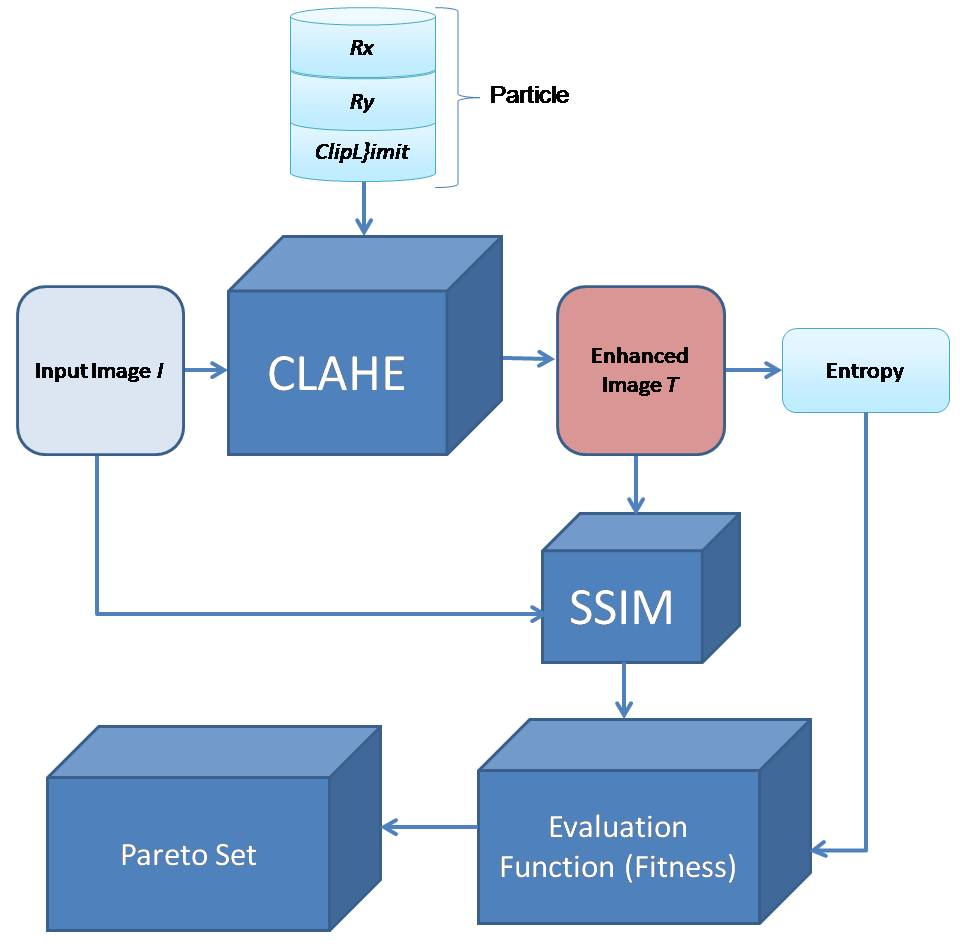
\includegraphics[height=6.5cm]{Figures/particula_clahe2.png}}
%   \vspace{0.5cm}
%   \label{fig:particula_clahe}
%   \captionof{figure}{Interacción entre CLAHE y SMPSO.}
% \end{minipage}

% \twocolumn
% \bibliographystyle{IEEEbib}
% \bibliography{refs}



\end{document}